% CORRELATION
\subsubsection{Correlation}
\label{subsection:corr}

The correlation of a linear filter $h(u,v)$ to an image $f(i,j)$ with the output $g(i,j)$ may be described mathematically as in Equation \ref{eq:correlation} but denoted more succinctly as in Equation \ref{eq:correlation_operator}

\begin{equation} \label{eq:correlation}
g(i,j) = \sum_{u=-k}^{k}\sum_{v = -l}^{l}f(i+u,j+v)h(u,v)
\end{equation}

\begin{equation} \label{eq:correlation_operator}
g = f \otimes h
\end{equation}

Correlation measures the \emph{similarity} between two signals and is used in image processing to measure the similarity between digital images and linear filters. Correlation produces output spikes not just where the image value is greatest because digital images and filters can contain negative values. For example a byte encoded grayscale image could be represented by [-127,128]. The significance of this is that when negative intensities are multiplied with other negative intensities they produce positive values and when negative values are multiplied with positive values they produce a negative, thus wherever a filter has the best match with the image a spike in positive values will occur and where the signals are dissimilar the output will be diminished \cite{optimalKernel}\cite{udacity_cv}. 

This simple method can be used to isolate features in an image by correlating an image with a filter that matches the desired feature. A feature could be as simple as a straight line or as specific as the outline of a car wheel. This method of feature detection is called \emph{template matching} \cite{oreilly_python}. In Figure \ref{fig:sobel_apply} vertical and horizontal Sobel filters are correlated with an image a building wall and produce images that emphasize lines that match the orientation of the respective filter (see section \ref{subsubsection:kernels}). The result is a binary image the output has been thresholded (see section \ref{subsection:thresholding}) to isolate high intensity regions where similarity is greatest.

% SOBEL FILTER APPLICATION
\begin{figure}[H]
  \centering
  \begin{subfigure}[b]{0.3\textwidth}
      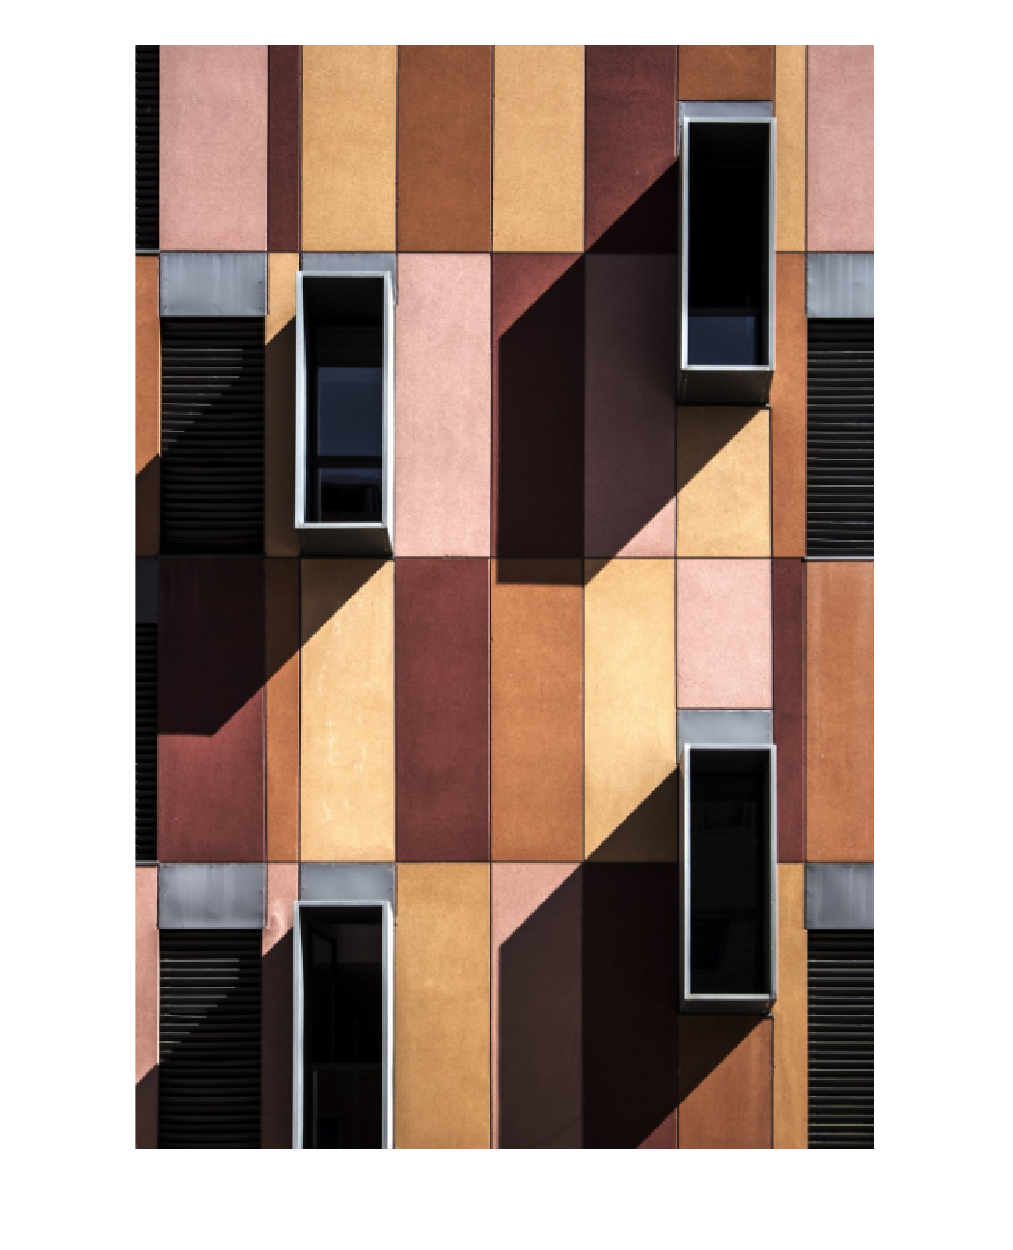
\includegraphics[width=\textwidth]{im_color}
      \caption{Img: Simone Hutsch}
  \end{subfigure}
  \begin{subfigure}[b]{0.3\textwidth}
      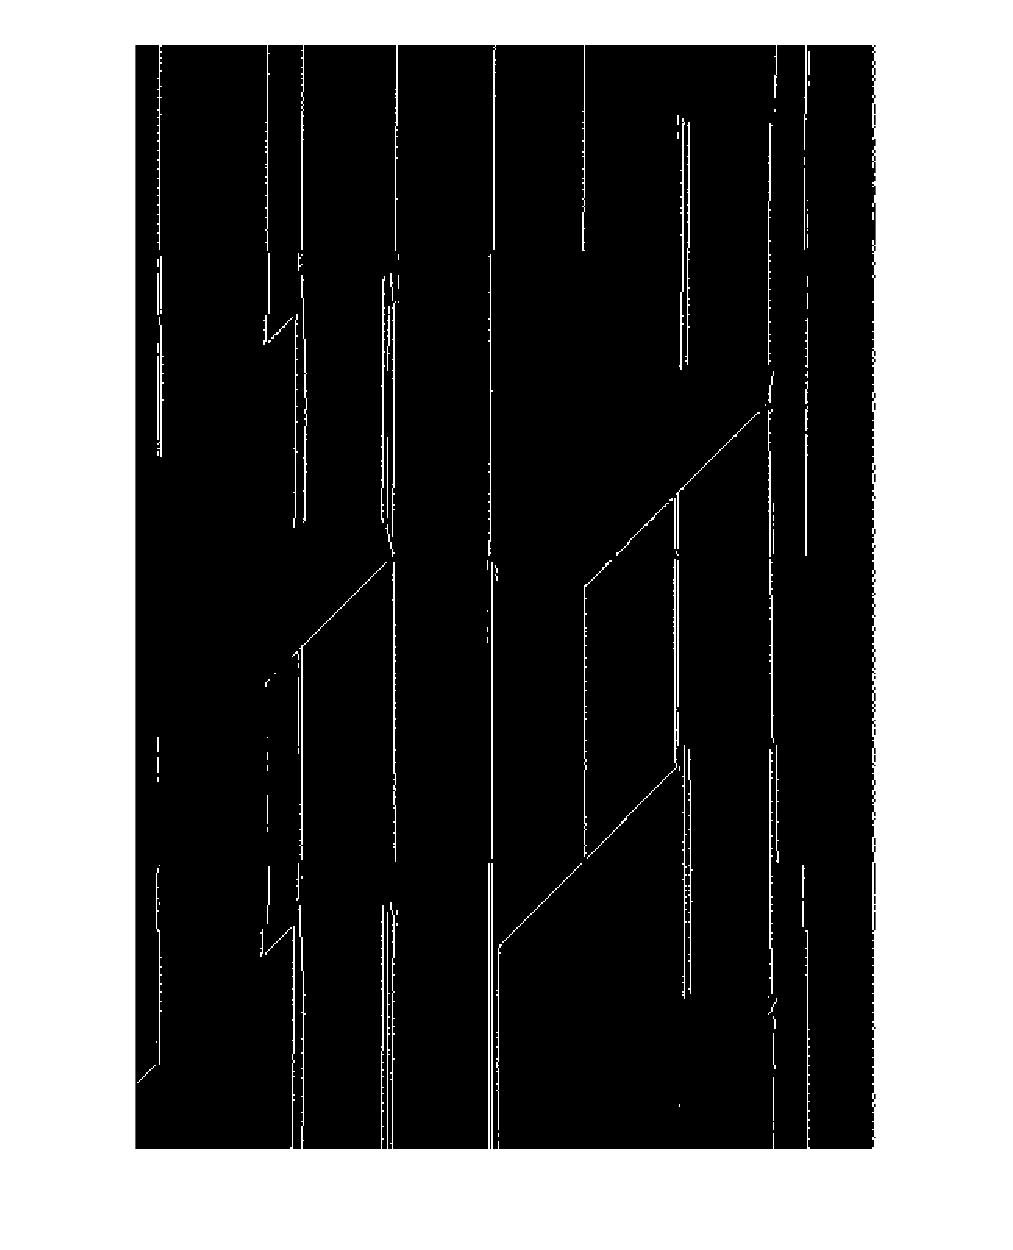
\includegraphics[width=\textwidth]{gv}
      \caption{Vertical similarity.}
      \label{fig:vert}
  \end{subfigure}
  \begin{subfigure}[b]{0.3\textwidth}
      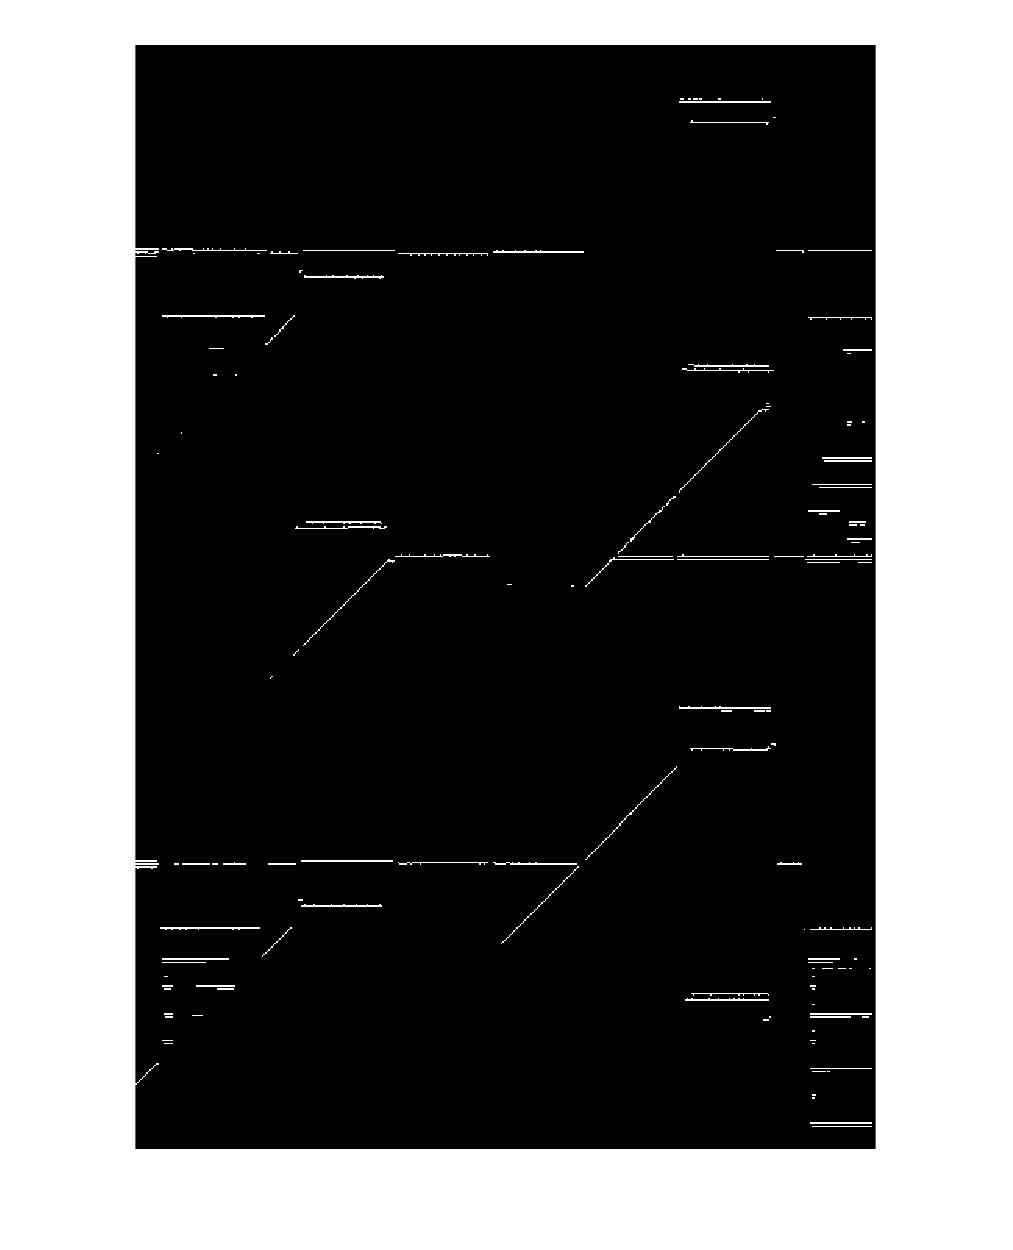
\includegraphics[width=\textwidth]{gh}
      \caption{Horizontal similarity.}
      \label{fig:hoz}
  \end{subfigure}
  \caption{Application of Sobel filters to exaggerate lines.}
  \label{fig:sobel_apply}
\end{figure}

In performing correlation at the edge of an image the portions of the filter can be outside the boundaries of the the image. To deal with this scenario an image can be prepared with \emph{padding} which adds additional pixels around the border of the image. There are many methods of padding an image such as mirroring which reflects pixels at the images edge into the new border and constant padding which just add a single colored border around the image \cite{realtimerendering}.

Correlation is a \emph{linear shift-invariant} (LSI) operator which means that it doesn't matter where a filter is correlated with an image or in what order it is applied to it's pixels, the result will be the same \cite{cv_matlab}. More formally an LSI operator satisfies the principals of super-positioning and shift invariance. Given a filter $h$ and signals $f_1$ and $f_2$ it doesn't matter whether the signals are added before they're filtered or the filter is applied individually and added the super-positioning principle states that the result is the same (equation \ref{eq:superpos}). The symbol $\circ$ represents the linear shift invariant operator).

\begin{equation}
  \label{eq:superpos}
  h\circ(f_1 + f_2) = h\circ f_1 + h\circ f_2
\end{equation}

The principal of shift invariance states that if the signal $g(i,j)$ is equal to the shifted signal $f(i+k,j+l)$ then these signals are still equivalent after the application of filter $h$ to both of them (equation \ref{eq:shiftinvariance}).

\begin{equation}
  \label{eq:shiftinvariance}
  g(i,j)=f(i+k,j+l) \Leftrightarrow\ (h\circ g)(i,j)=(h\circ f)(i+k,j+l)
\end{equation}

Figure \ref{fig:correlation} demonstrates a side effect of correlation which is to flip both horizontally and vertically the output signal relative to the the original image \cite{udacity_cv}. This occurs because as a filter scans over an image the output of the neighborhood is stored at the filter's origin. This effect can be negated by flipping the filter in both directions before applying it to the signal and is the only difference between correlation and convolution. This difference means however that in convolution the similarity between signals is not been measure but the effect one signal has on another. The next section covers convolution in greater detail.

% CORRELATION EXAMPLE  %
\begin{figure}[H] 
  \centering
  \begin{tabular}{ccccc}
      \begin{tabular}{|c|c|c|c|c|}
      \hline
      0 & 0 & 0 & 0 & 0 \\[1pt]
      \hline
      0 & 0 & 0 & 0 & 0 \\[1pt]
      \hline
      0 & 0 & 1 & 0 & 0 \\[1pt]
      \hline
      0 & 0 & 0 & 0 & 0 \\[1pt]
      \hline
      0 & 0 & 0 & 0 & 0 \\[1pt]
      \hline
      \end{tabular}%
    & $\otimes$ &
    \begin{tabular}{|c|c|c|}
      \hline
      a & b & c \\
      \hline
      d & e & f \\
      \hline
      g & h & i \\
      \hline 
    \end{tabular}
    & $=$ &
    \begin{tabular}{|c|c|c|c|c|}
      \hline
      0 & 0 & 0 & 0 & 0 \\[1pt]
      \hline
      0 & \textbf{i} & \textbf{h} & \textbf{g} & 0 \\[1pt]
      \hline
      0 & \textbf{f} & \textbf{e} & \textbf{d} & 0 \\[1pt]
      \hline
      0 & \textbf{c} & \textbf{b} & \textbf{a} & 0 \\[1pt]
      \hline
      0 & 0 & 0 & 0 & 0 \\[1pt]
      \hline
    \end{tabular} \\
    $F(x,y)$ & & $H(u,v)$& & $G(x,y)$ \\
  \end{tabular}
  \caption{Correlation of a filter and an image.}
  \label{fig:correlation}
\end{figure}